
\section{SRIM}

The SRIM/TRIM computer code was used to simulate ions within the target material.

The composition of the material is input into the SRIM graphical interface.  As the activity code currently works for proton projectiles only, and the experimental work was completed with protons, this is chosen as the projectile in SRIM.  Finally, the projectile energy is selected



\begin{center}
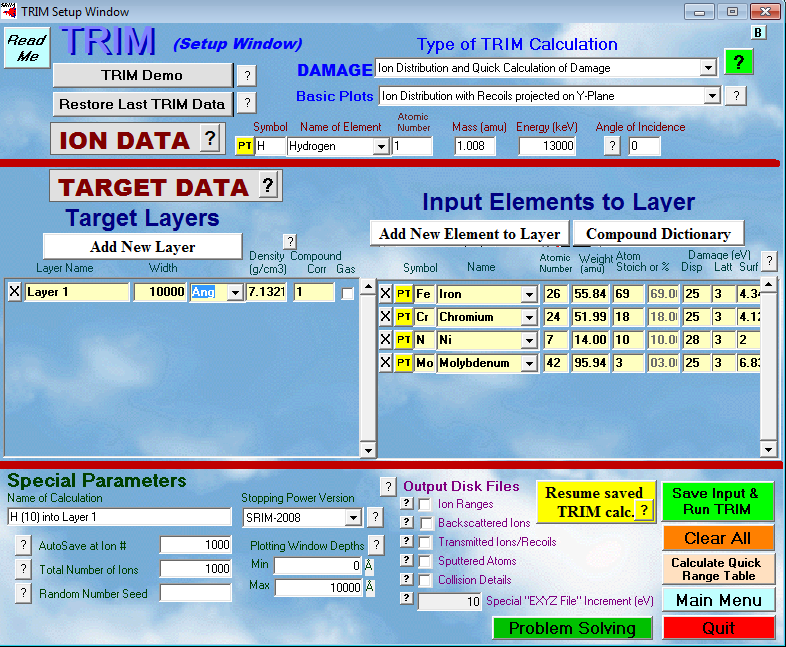
\includegraphics[scale=0.35]{chapters/methodology_activity/images/trim.png}
\end{center}




